

\chapter{設計と実装}
\label{chap:system}
本章では前章の最後に述べた「読者側の操作で閲覧環境に則り,視認性の高い文章レイアウトを再形成するアプローチ」
の定義を明確にした上で,その実装形態である「ReaderLint」の要件と設計について述べる.
\newpage

\section{システムの定義}
これまで示してきた文章レイアウトの問題を解決するための要件は以下の4つであると仮定し,設計を行なった.
\begin{enumerate}
	\item 文章のリーダビリティの研究に基づき,読み手側のデバイスに向上させる改行を行う.
	\item 書き手側のつけた改行が文章の段落位置が読み手側から見たときに可読性を損ねていた場合には操作を行う.
	\item 文章内のリンク,emojiといった装飾を破壊しない.
	\item 1, 2, 3を踏まえた上で書き手側の意図(改行による段落生成など),書き手側の文意を損ねることなく行う
\end{enumerate}
2.の改行箇所が可読性を損ねている,という判定に関しては本研究では行頭から2~3文字後に改行が行われ,
文章レイアウトに凸凹ができている場合,という想定のもと実装を行なった.上記の4つの要件を踏まえた上でシステムの機能と実装を記す.

\section{ReaderLintの機能}
ReaderLintはブラウザ上にレンダリングされている文章に対し,文章の折り返し地点が文節として不可分,一文節の途中であった場合,
その文節前に改行処理を加えることで,文節間を検知した改行レイアウトを自動的に改稿を行うシステムである.
処理をかける文章はデバイス内のDOMにレンダリングされた文章なのでその表示環境に応じた改行レイアウト処理を行うことができる.
勿論,これは自身の画面での表示環境に応じて一時的に文章レイアウトを変更しているため,閲読しているページを更新すれば改稿前の文章に戻り,
画面サイズの異なる他のデバイスで行なった場合にまた異なる改行レイアウトとなる.
一方で,ReaderLintを使用している状態で画面サイズをリサイズした場合にはリサイズ後のDOMサイズに対応した改行レイアウトをレンダリングする.
前章の『Web上の文章の特色』にて述べた[句点代わりに行われる改行を用いたレイアウト」を取り入れている場合,読み手側ので表示される文章レイアウトにて
開業による大きな凹凸があると判定された場合は改行を再度行い,違和感を緩和する機能を入れている.

\begin{figure}[H]
    \centering
    \label{fig:image11}
    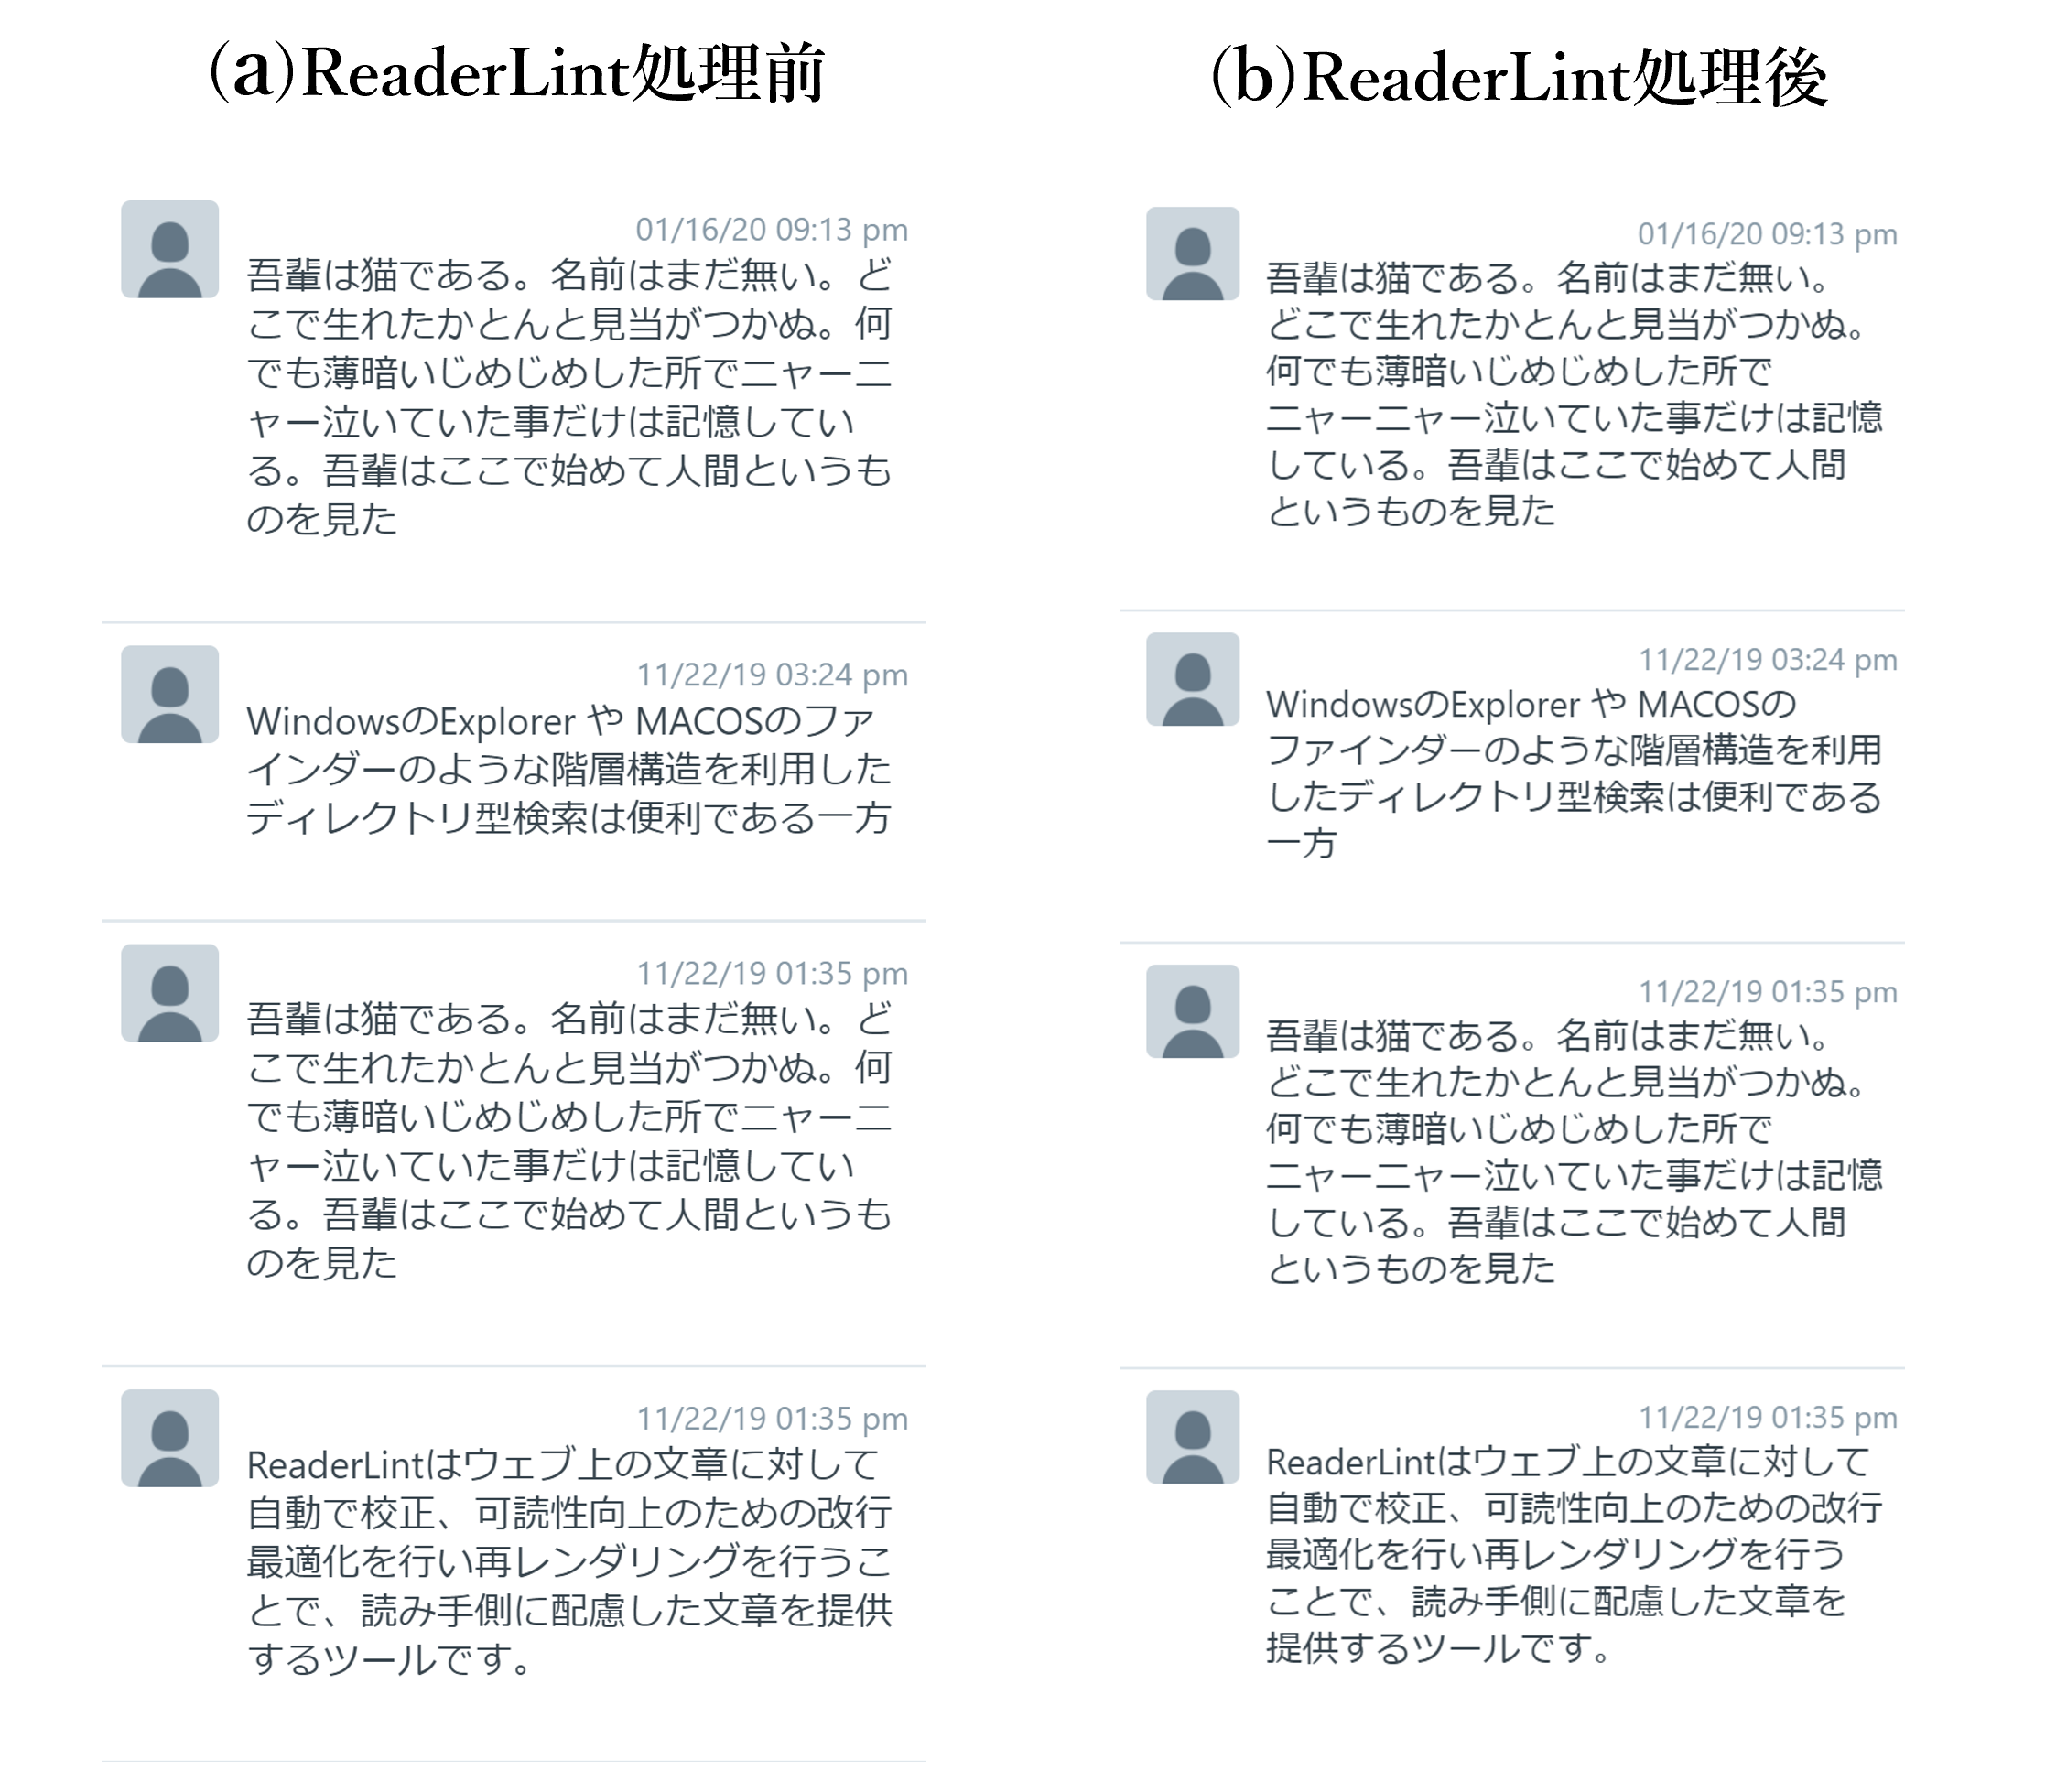
\includegraphics[width=0.7\columnwidth]{image/03/img2.png}
    \caption[文章の再形成が行われた画面]{文章の再形成が行われた画面\footnotemark[1]}
\end{figure}

\footnotetext[1]{
    ツイート文章は夏目漱石『吾輩は猫である』\cite{夏目}より引用
}

\section{基本構成}

本システムはGoogle社の提供するブラウザであるChrome拡張機能としてJavaScript製で実装されている.
Chromeではブラウザの拡張機能をサードパーティーアプリとしてインストールすることが可能であり,
自作のJavaScript製のコードをインストールすることで拡張機能としてブラウザ内で使用することができる.
ReaderLintはこのChormeの拡張機能としてインストールして使用できる.

ReaderLintのインストール後には左クリックでコンテキストメニュー上に表示され,
メニューをクリックするとReaderLintを実行するDOMを選択できる状態になる.
この状態でテキストが挿入されているDOMをクリックすると指定したDOM内のHTML要素からテキスト箇所の
解析を行い,処理を行なったテキストを反映する.上記処理をすべてクライアントサイドのみでサーバー処理を
挟まずに稼働する実装となっている.

\begin{figure}[H]
    \centering
    \label{fig:context}
    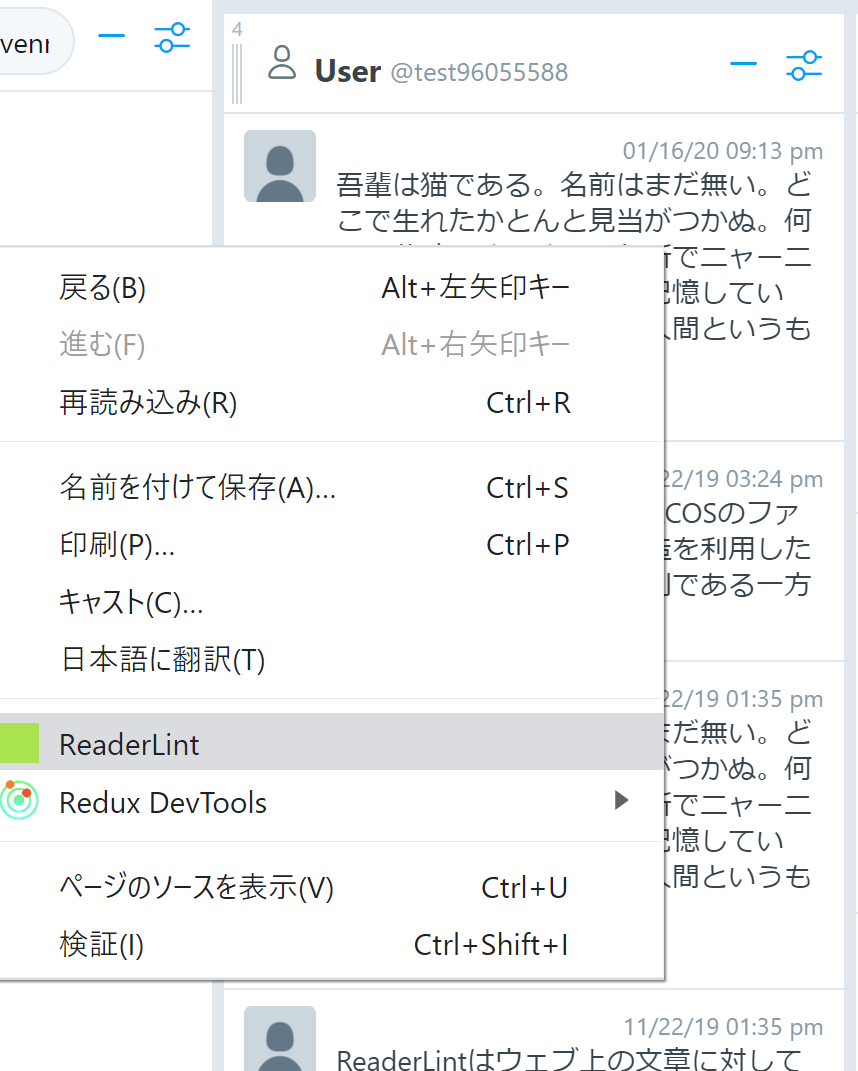
\includegraphics[width=0.4\columnwidth]{image/03/img0.png}
    \caption[コンテキストメニュー]{コンテキストメニュー}
\end{figure}

また,視認性の理由から文章の格納されているDOMのサイズが900pxを超えている場合には,
900pxに収まるよう調整をかけている.以下の画像は横幅が1345pxであった
DOMの文章にReaderLintを実行した際の動作である.\footnotemark[2]

\footnotetext[2]{参考: 
	\protect\url {https://anond.hatelabo.jp/20200112130927}
}

\begin{figure}[H]
    \centering
    \label{fig:image12}
    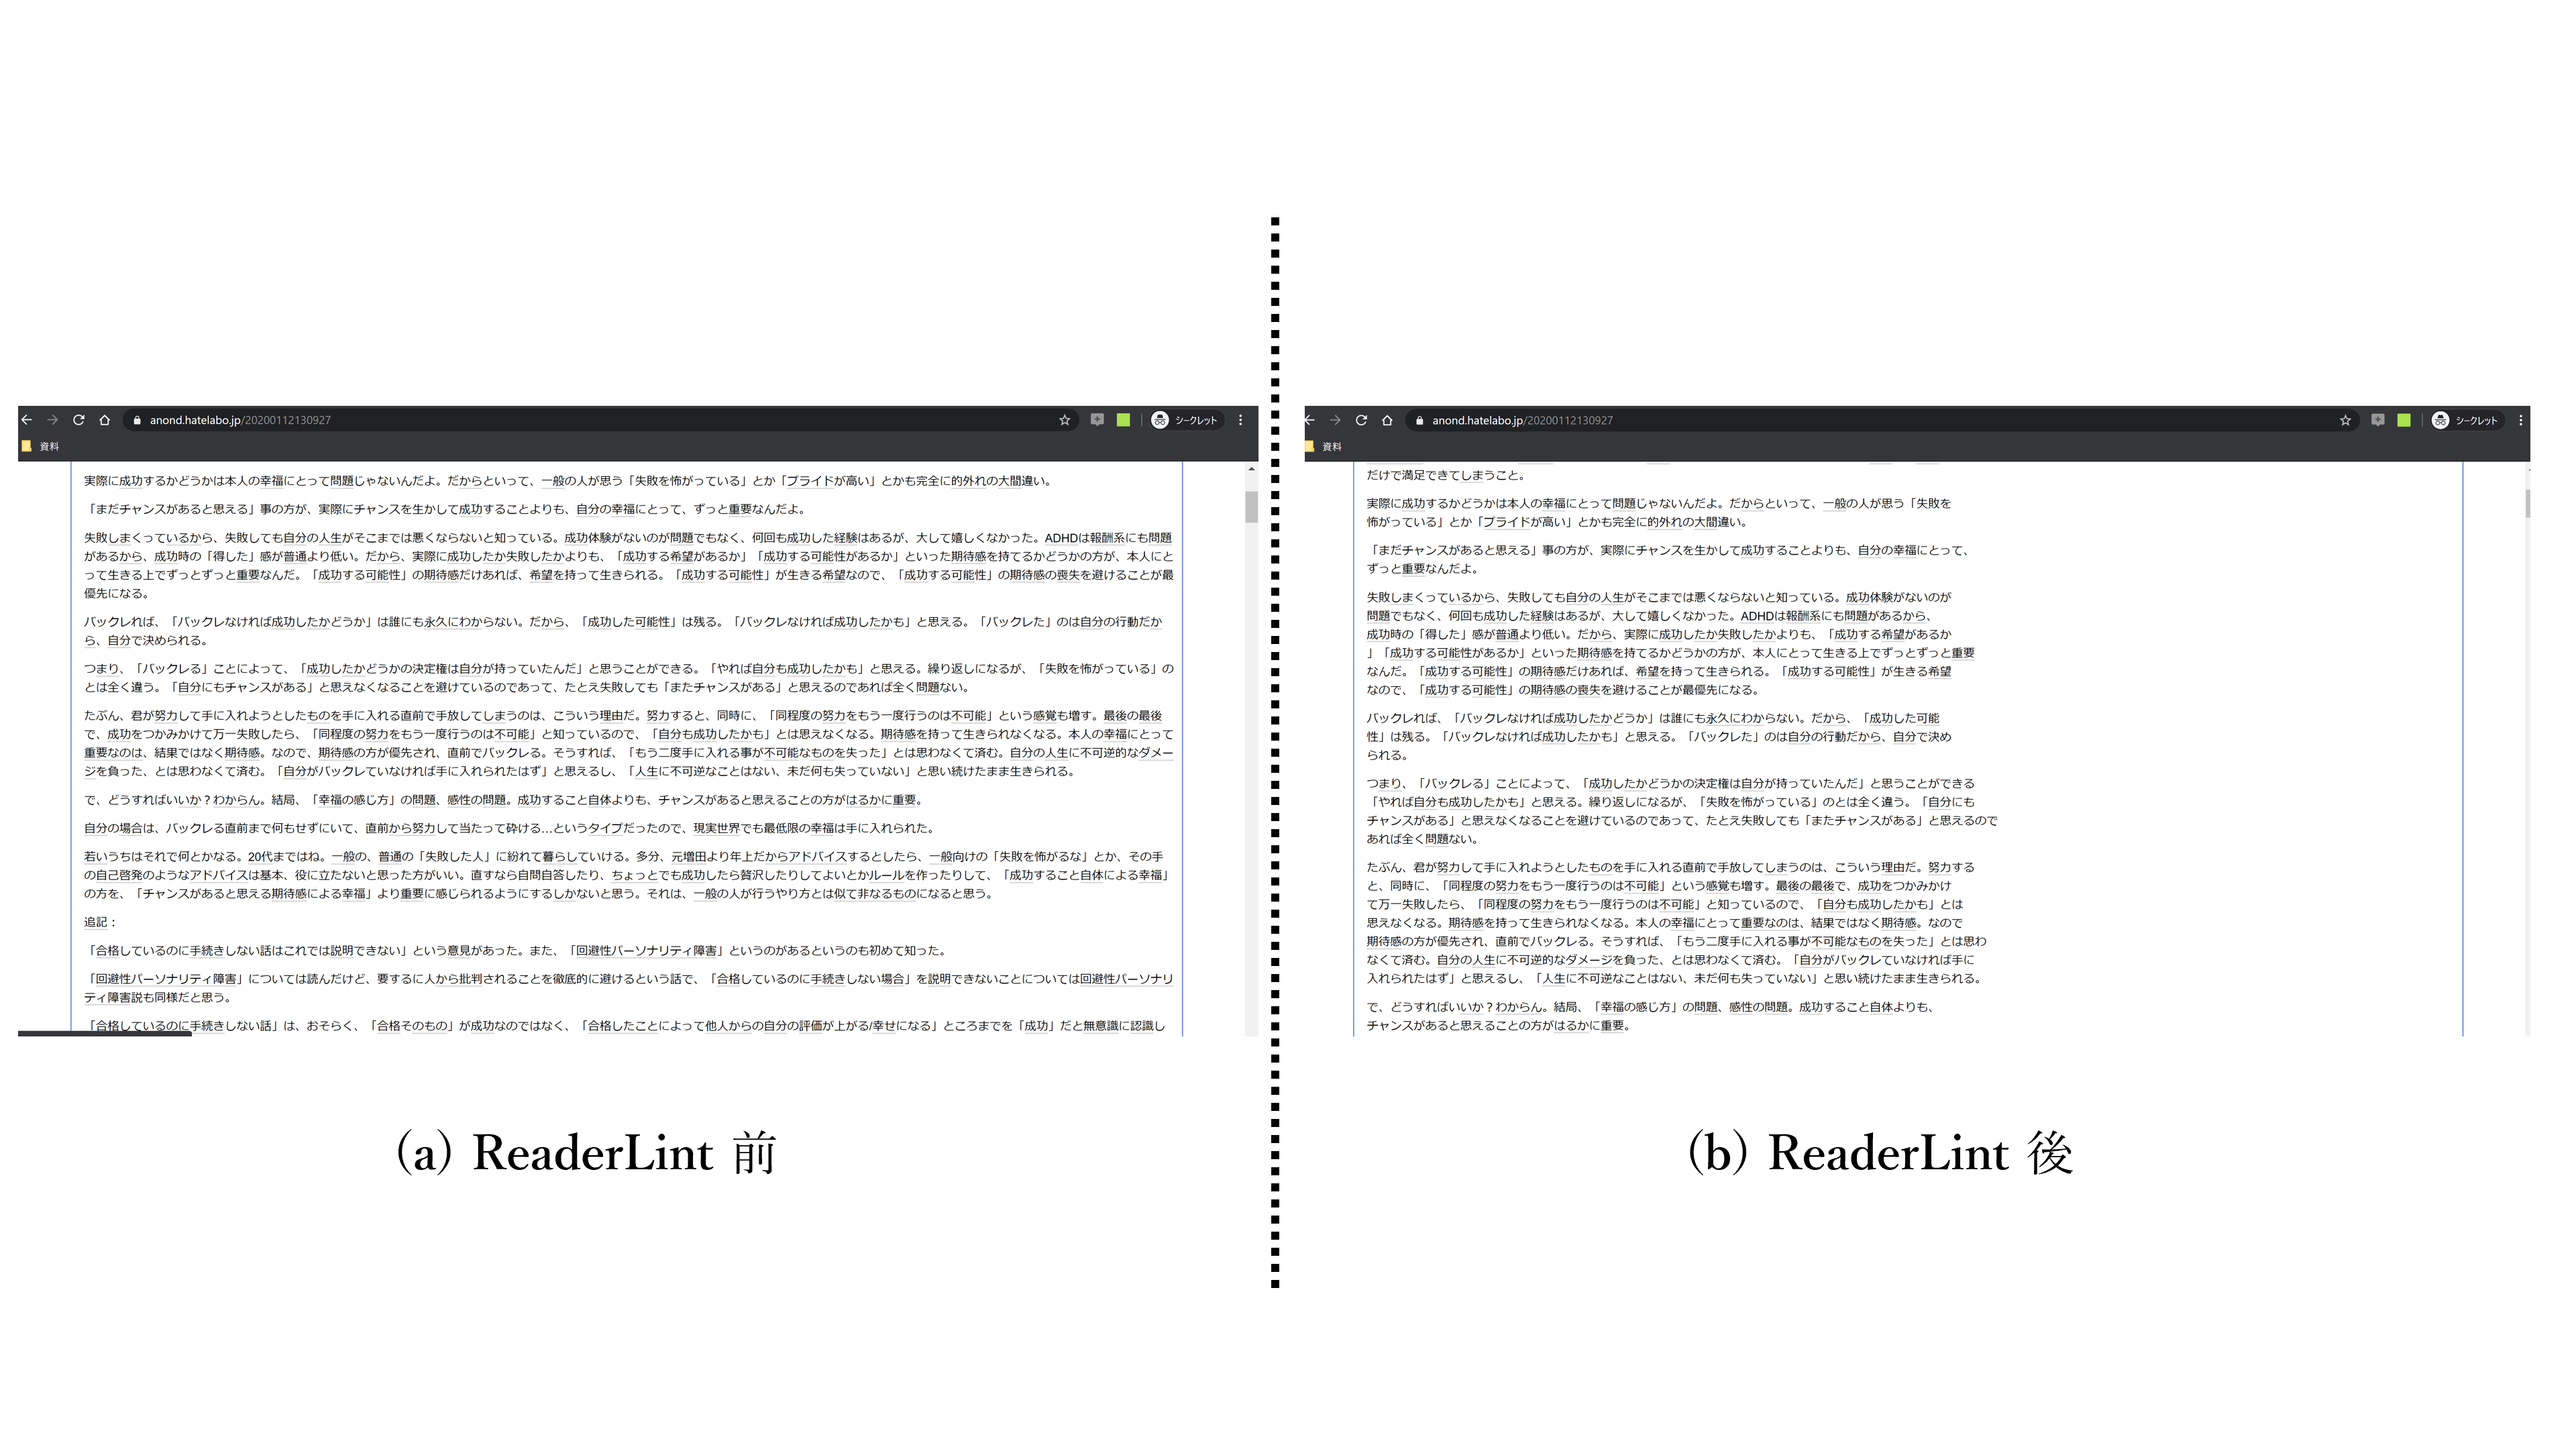
\includegraphics[width=0.8\columnwidth]{image/03/img8.png}
	\caption[幅の大きいDOMに対して施行後]{横幅の大きいDOMに対して施行後}
\end{figure}

\section{実装}

\subsection{DOMの取得}
ReaderLintを実行するDOMの取得には,コンテキストメニューをクリックした後,
document.elementFromPointによりカーソルがホバーしているDOMを検出が可能となる.その状態でクリックしたDOMの横幅が100px以上であり,
かつ読み手側のブラウザで文章が表示されているか(elenment.textContentとして文章が取得が可能か)を判定し,それらを満たしていた場合に,
取得を行なう.この際に指定したDOMの親タグ,およびそのDOMにかかっているclass名から,対象となりえるDOMを取得する.
1つのDOMにて処理が終わったあとには対象DOMを巡回してReaderLintを実行するという実装を行なった

\begin{figure}[H]
    \centering
    \label{fig:image10}
    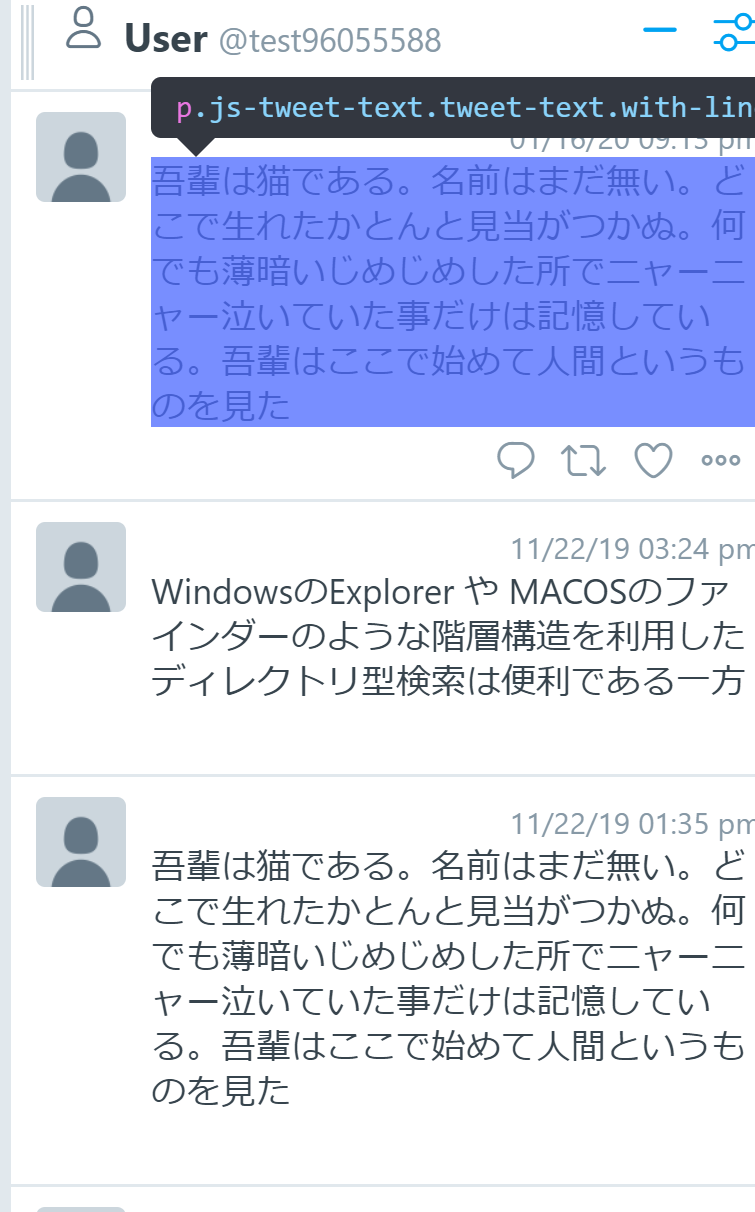
\includegraphics[width=0.7\columnwidth]{image/03/img1.png}
    \caption[DOM選択モード] {DOM選択モード}
\end{figure}

\subsection{文章の折返し箇所の自動検出}
文節ごとに区切られた改行を行うためには,左詰から開始された文章の一行の横幅が指定したDOMの横幅(width)を超える文字,
文章の折返し箇所を検知する必要がある.現在のWebAPIには日本語の文章を折り返す文字の箇所を自動検知できる,といった仕様は存在しない.
そのため,一度文章全体に文節ごとに分かち書きを行い,文節ごとに描画幅を計測し,分かれた文字列を文章での並び順に
配列として格納,一行に含まれる文節ごとの描画幅の総和がDOMサイズを超過した際に,その文節の前に改行文字を挿入し配列に加える,
という検知方法を採用した.最後に完成した配列を連結させ,文字列として元のDOMのinnerHTMLに返すことで処理を加えたテキストを反映させた.
以下は文章の分かち書きを行なった際の分かれ方の一例と文節間改行レイアウトのイメージである.

\begin{verbatim} ["吾輩","は","猫","で","ある","。", "名前","は","まだ","無い","。", …]
\end{verbatim}

\begin{figure}[H]
    \centering
    \label{fig:image14}
    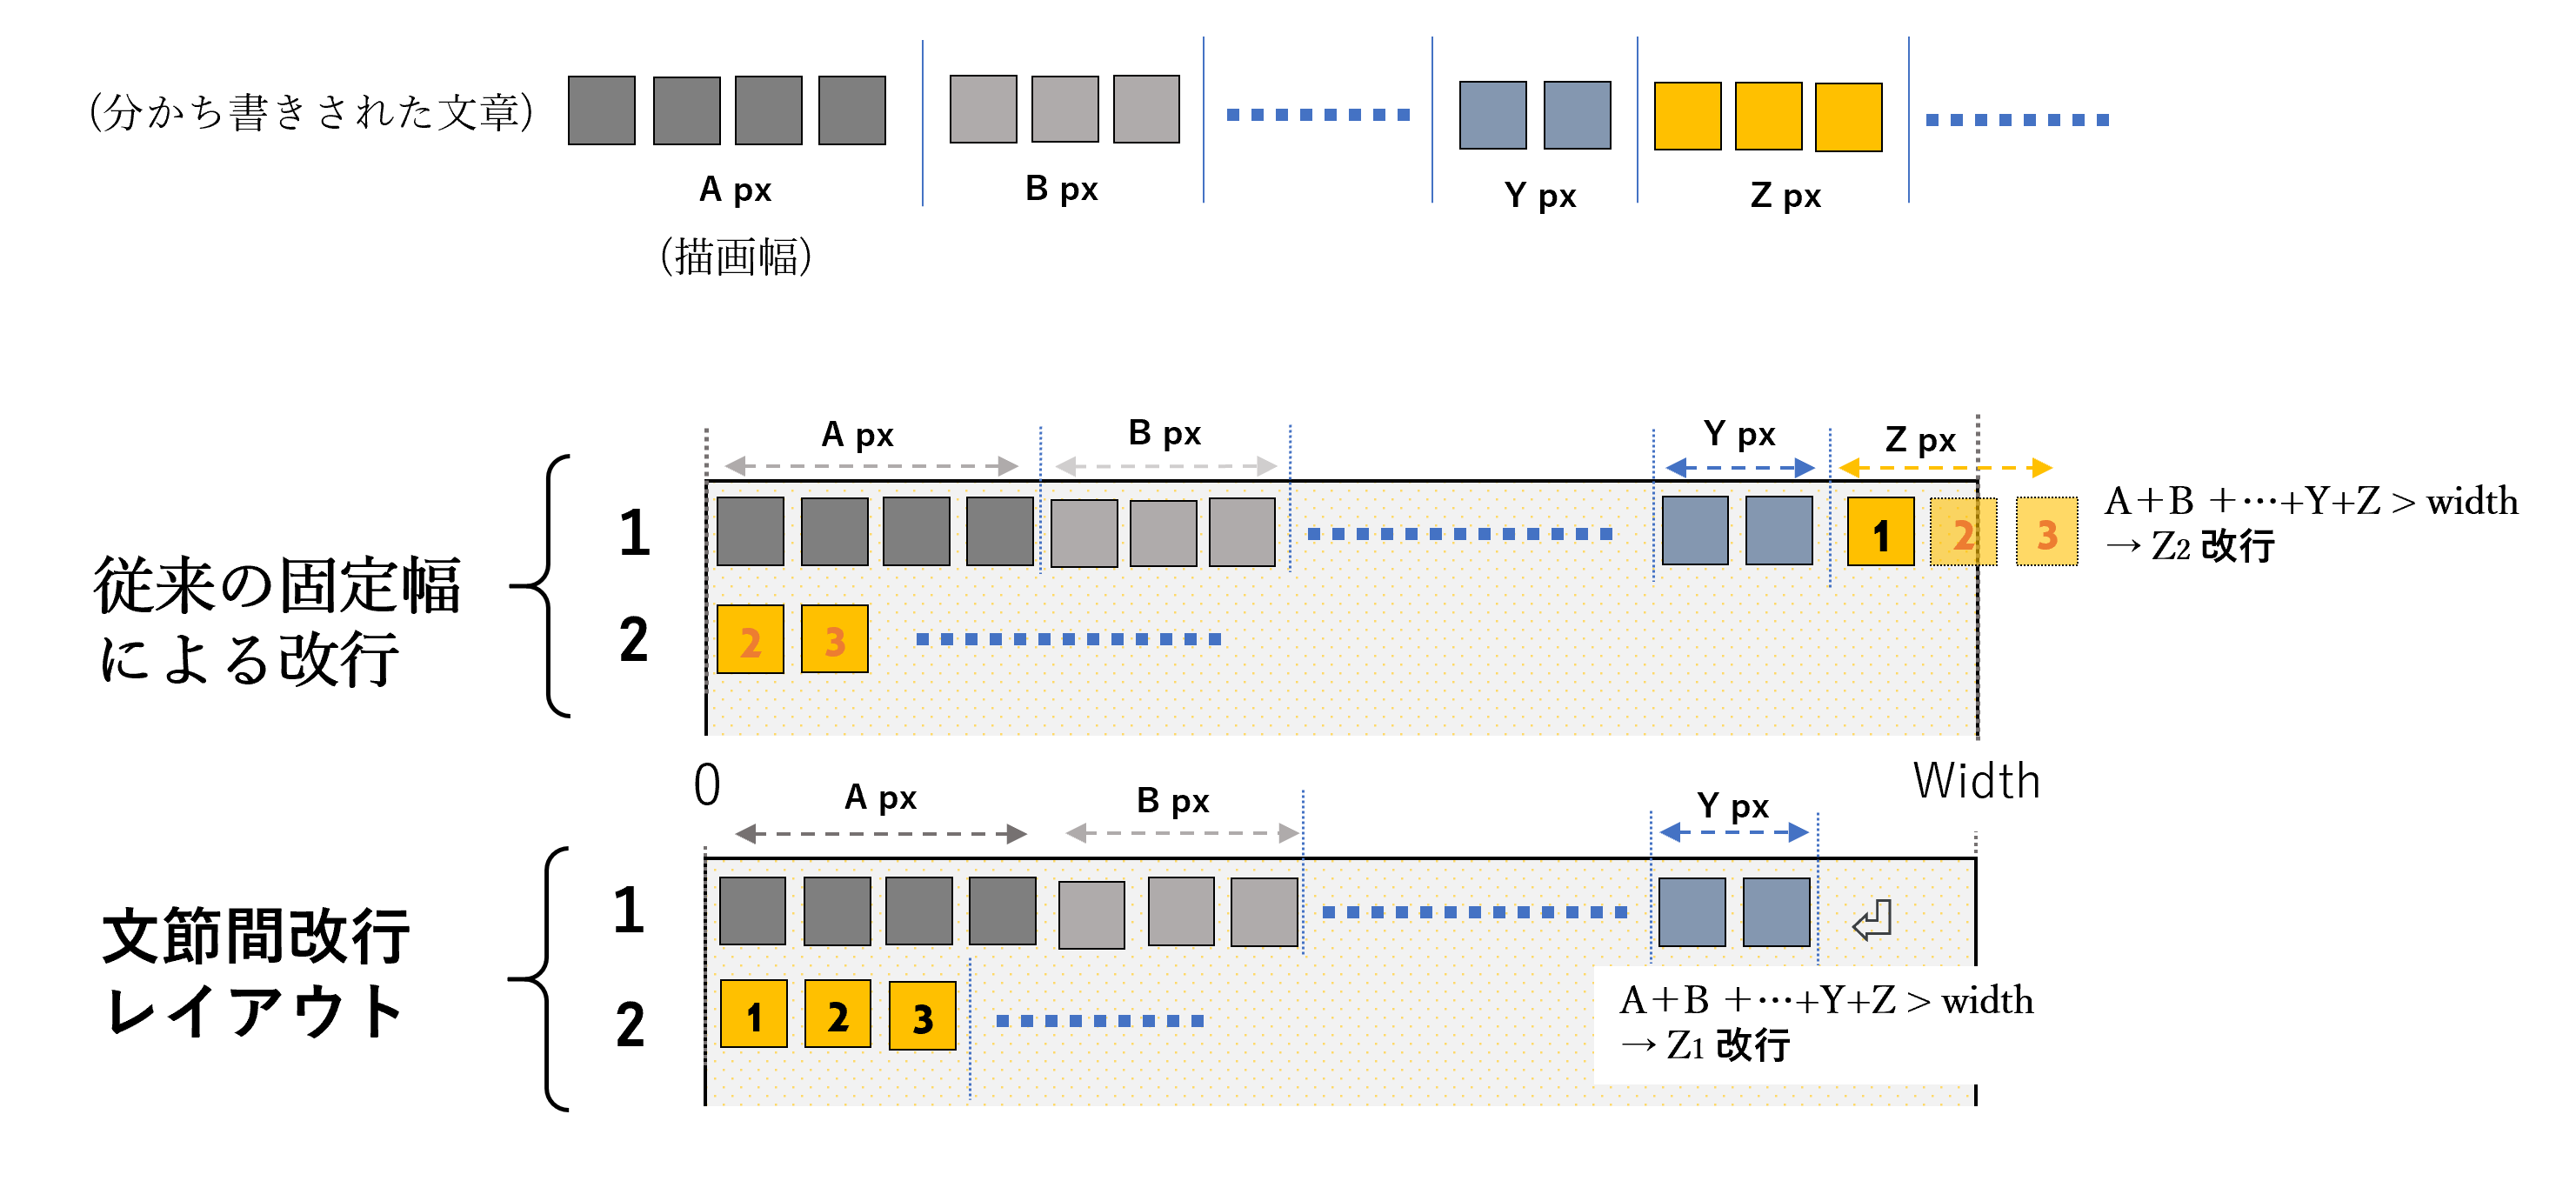
\includegraphics[width=0.6\columnwidth]{image/03/img6.png}
	\caption[文節ごとの改行処理]{文節ごとの改行処理]}
\end{figure}

この方法を実装するには日本語の分かち書きにより文節ごとに分け,および各文節の描画幅を予測することが必要となる.
この処理を行なうために用いた方法として以下の2つを紹介する.

\subsubsection{日本語分かち書き}
文章に対して文節ごとに区切る分かち書きの,文章を文節ごとに区切る,といった日本語分かち書きを行うライブラリには
辞書ベースのデータに頼る辞書データ型と,大まかな解析データに頼る辞書なし型の2つに大別される.
今回は辞書なし型であるTinySegmenterを用いた.TinySegmenterとは工藤匠氏が開発し,
公開しているJavaScript製の日本語分かち書きライブラリである.\footnotemark[3]
TinySegmenterには以下の特色がある.

\begin{enumerate}
	\item JavaScript製であり,クライアントサイドに組み込むだけで分かち書き処理が可能である点
	\item 機械学習のみで辞書データに非依存的であるため,辞書データを用いたものと比較した際に次女のロード時間がなく,高速で分かち書き処理を行う点
	\item 25キロバイトという軽量さ
	\item くだけた文章表現には弱い一方,辞書データに依存しないため,登録されていない未知語に対して検出率が高い点
\end{enumerate}
TinySegmenterはあくまで新聞文章のデータコーパスから機械学習を行なったモデルをもとに分かち書き処理を行うため,
辞書データを用いたものよりもよりも分かち書きの精度は低いとされているが,上記の利点を加味して採用した.

\footnotetext[3]{
	参照: \protect\url {http://chasen.org/~taku/software/TinySegmenter/}
}

\subsubsection{canvas要素を用いた文字幅の計測}
canvasとはHTML5にて追加されたHTML上にてビッドマップキャンバスを用いた視覚的な画像をレンダリングすることを目的とした
HTML要素である.canvasが提供する機能のうち2DcontextAPI.measureTextメソッドはcanvas上でレンダリングするテキストの描画幅を測定し,
ピクセル単位で返してくれるメソッドである.描画幅としては指定したフォントでテキストを描画した場合の描画幅を返してくれるため,
文章を格納しているDOMのフォント設定とフォントサイズを設定すれば,DOMにてレンダリングされている文字幅の数値のシミュレートが可能となる.
今回は仮想的なcanvas要素を設定し,そこに描画幅を計測する文章を設定することで文章の描画幅の計測を試みた.

改行レイアウトのアルゴリズムは上記の2つを用いて,文節ごとの描画幅を計測することで実装した.

\subsection{ASTを用いた文章解析}
対象として選んだ文章にはDOMの内部にはリンク,画像,改行といった平文以外の文字列が存在するため,
あらかじめ文章の種類を分別する前処理を挟んだ上で,改行レイアウト処理を行う必要があった.
文章の種類を分別する手法として,今回はAST\footnotemark[4]を用いる.
ASTとは本来はプログラミング言語の静的解析やそれに基づいた処理を行う際に文字列からパースされるデータ構造である.
データ構造としてあらかじめ文章の種類を分けたうえで,その種類ごとに加える編集を分ける,
という前処理を行なった.以下はASTとして処理された文章をJSON形式で出力したものを簡略化して表示したものである.

\footnotetext[4]{
    Abstract Syntax Tree, 抽象木構造
}

\newpage
\begin{figure}[H]
    \centering
    \label{fig:ASTofBreak}
    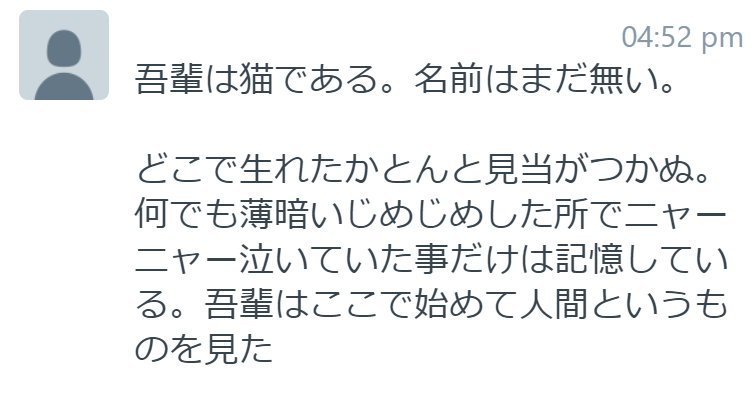
\includegraphics[width=0.6\columnwidth]{image/03/breakAST.png}
	\caption[ASTによるBreak検知例]{ASTによるBreak検知例}
\end{figure}

\begin{lstlisting}[caption=textToAST.json]
    {
        "children": [
            {
                "type": "Str",
                "raw": "吾輩は猫である.名前はまだ無い.",
                "value": "吾輩は猫である.名前はまだ無い.",
                "range": [
                    0,
                    16
                ],
                "loc": {
                    "start": {
                        "line": 1,
                        "column": 0
                    },
                    "end": {
                        "line": 1,
                        "column": 16
                    }
                }
            }
        ]
    },
    {
        "type": "Break",
        "raw": "\n",
        "value": "\n",
        "range":[
            16,
            17
        ],
        "loc": {
            "start": {
                "line": 1,
                "column": 16
            },
            "end": {
                "line": 1,
                "column": 17
            }
        }
    },
    ...
\end{lstlisting}

今回利用したASTライブラリは,実際に文章としてレンダリングされた箇所と,DOM内で記述されるHTMLタグの内容とを分別して
ASTを出力するtextlint/markdown-to-astに改行箇所を示すエスケープシーケンス $\backslash$n
を検知する仕様に変更したものと\footnotemark[5],AST化した文章の種類ごとにその文字列に施す処理を記述できるtextlint/ast-to-traverseを使用した.\footnotemark[6]

\footnotetext[5]{\protect\url{https://github.com/textlint/textlint/tree/master/packages/@textlint/markdown-to-ast}}
\footnotetext[6]{\protect\url{https://github.com/textlint/textlint/tree/master/packages/@textlint/ast-traverse}}

ASTによって文章をデータ構造としてパースする前処理の利点は,ブラウザ上にレンダリングされているリンクやハッシュタグ,
といったHTML要素に由来する表記を非破壊的に監査できる点にある.HTMLタグの中身である文章としてレンダリングされている
箇所だけを文節として取り出し描画幅を計測し加算を行なった上で配列にHTMLごとを格納することで,挿入されたHTMLタグ内の文字列に
改行コードを入れてHTML要素を破壊してしまうことを防止した.以下は文字に埋め込まれたURLリンクと文字とを判別した
ASTを簡略化して表示した図である。

\begin{figure}[H]
    \centering
    \label{fig:image16}
    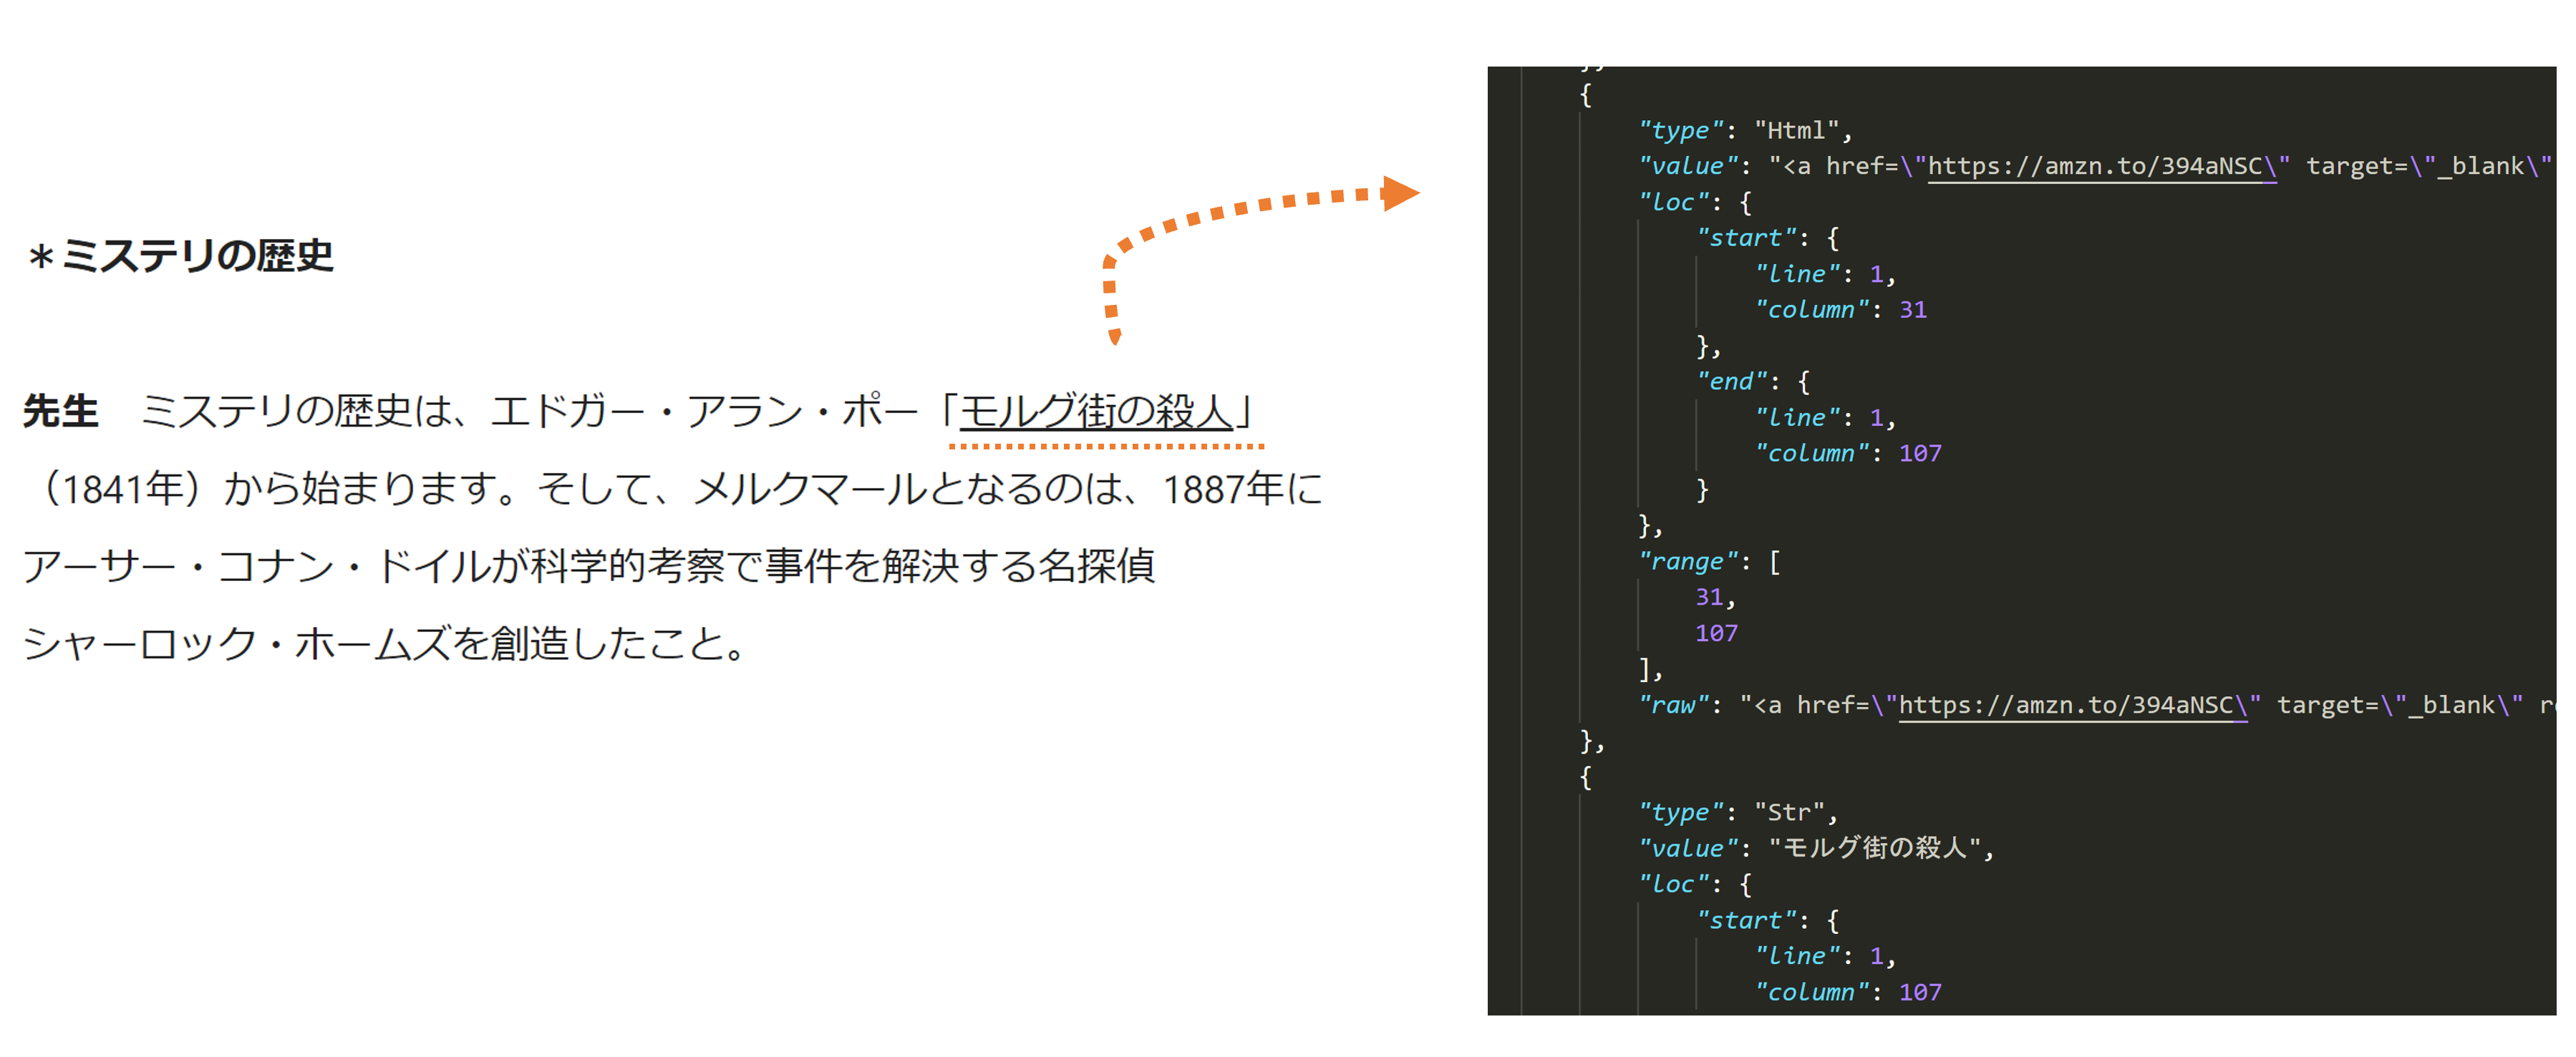
\includegraphics[width=0.7\columnwidth]{image/03/img7.png}
	\caption[HTMLタグ内の文章を分けて処理する図]{HTMLタグ内の文章を分けて処理する図} \footnotemark[7]
\end{figure}

\footnotetext[7]{使用サイト:\protect\url{https://www.hayakawabooks.com/n/ncdfb31dc4e46?creator_urlname=hayakawashobo01}}

\begin{lstlisting}{AST.json}
    {
         "type": "Html",
         "value": "<a href=\"https://amzn.to/394aNSC\" target=\"_blank\" rel=\"noopener noreferrer\">",
            …
         "raw": "<a href=\"https://amzn.to/394aNSC\" target=\"_blank\" rel=\"noopener noreferrer\">"
     },
     {
         "type": "Str",
         "value": "モルグ街の殺人",
            …
         "raw": "モルグ街の殺人"
    }
\end{lstlisting}

\subsection{視認性を損ねた改行位置の処理}
視認性を損ねる箇所で行わる改行に関しては,ASTで改行を検知し,行数が更新されたタイミングから行頭から改行が行なわれるまでの描画幅の総和が設定した規定値
以下だった場合には文章を詰める,または文章を段落的に分けるという処理が可能となっている.
以下の画像はReaderLintの処理後に文頭から文末までの描画幅がDOMの横幅の2割以下だった場合にのみ改行を解除し,前文節に半空白をうち,字詰めを行なった例である.

\begin{figure}[H]
    \centering
    \label{fig:jutsume}
    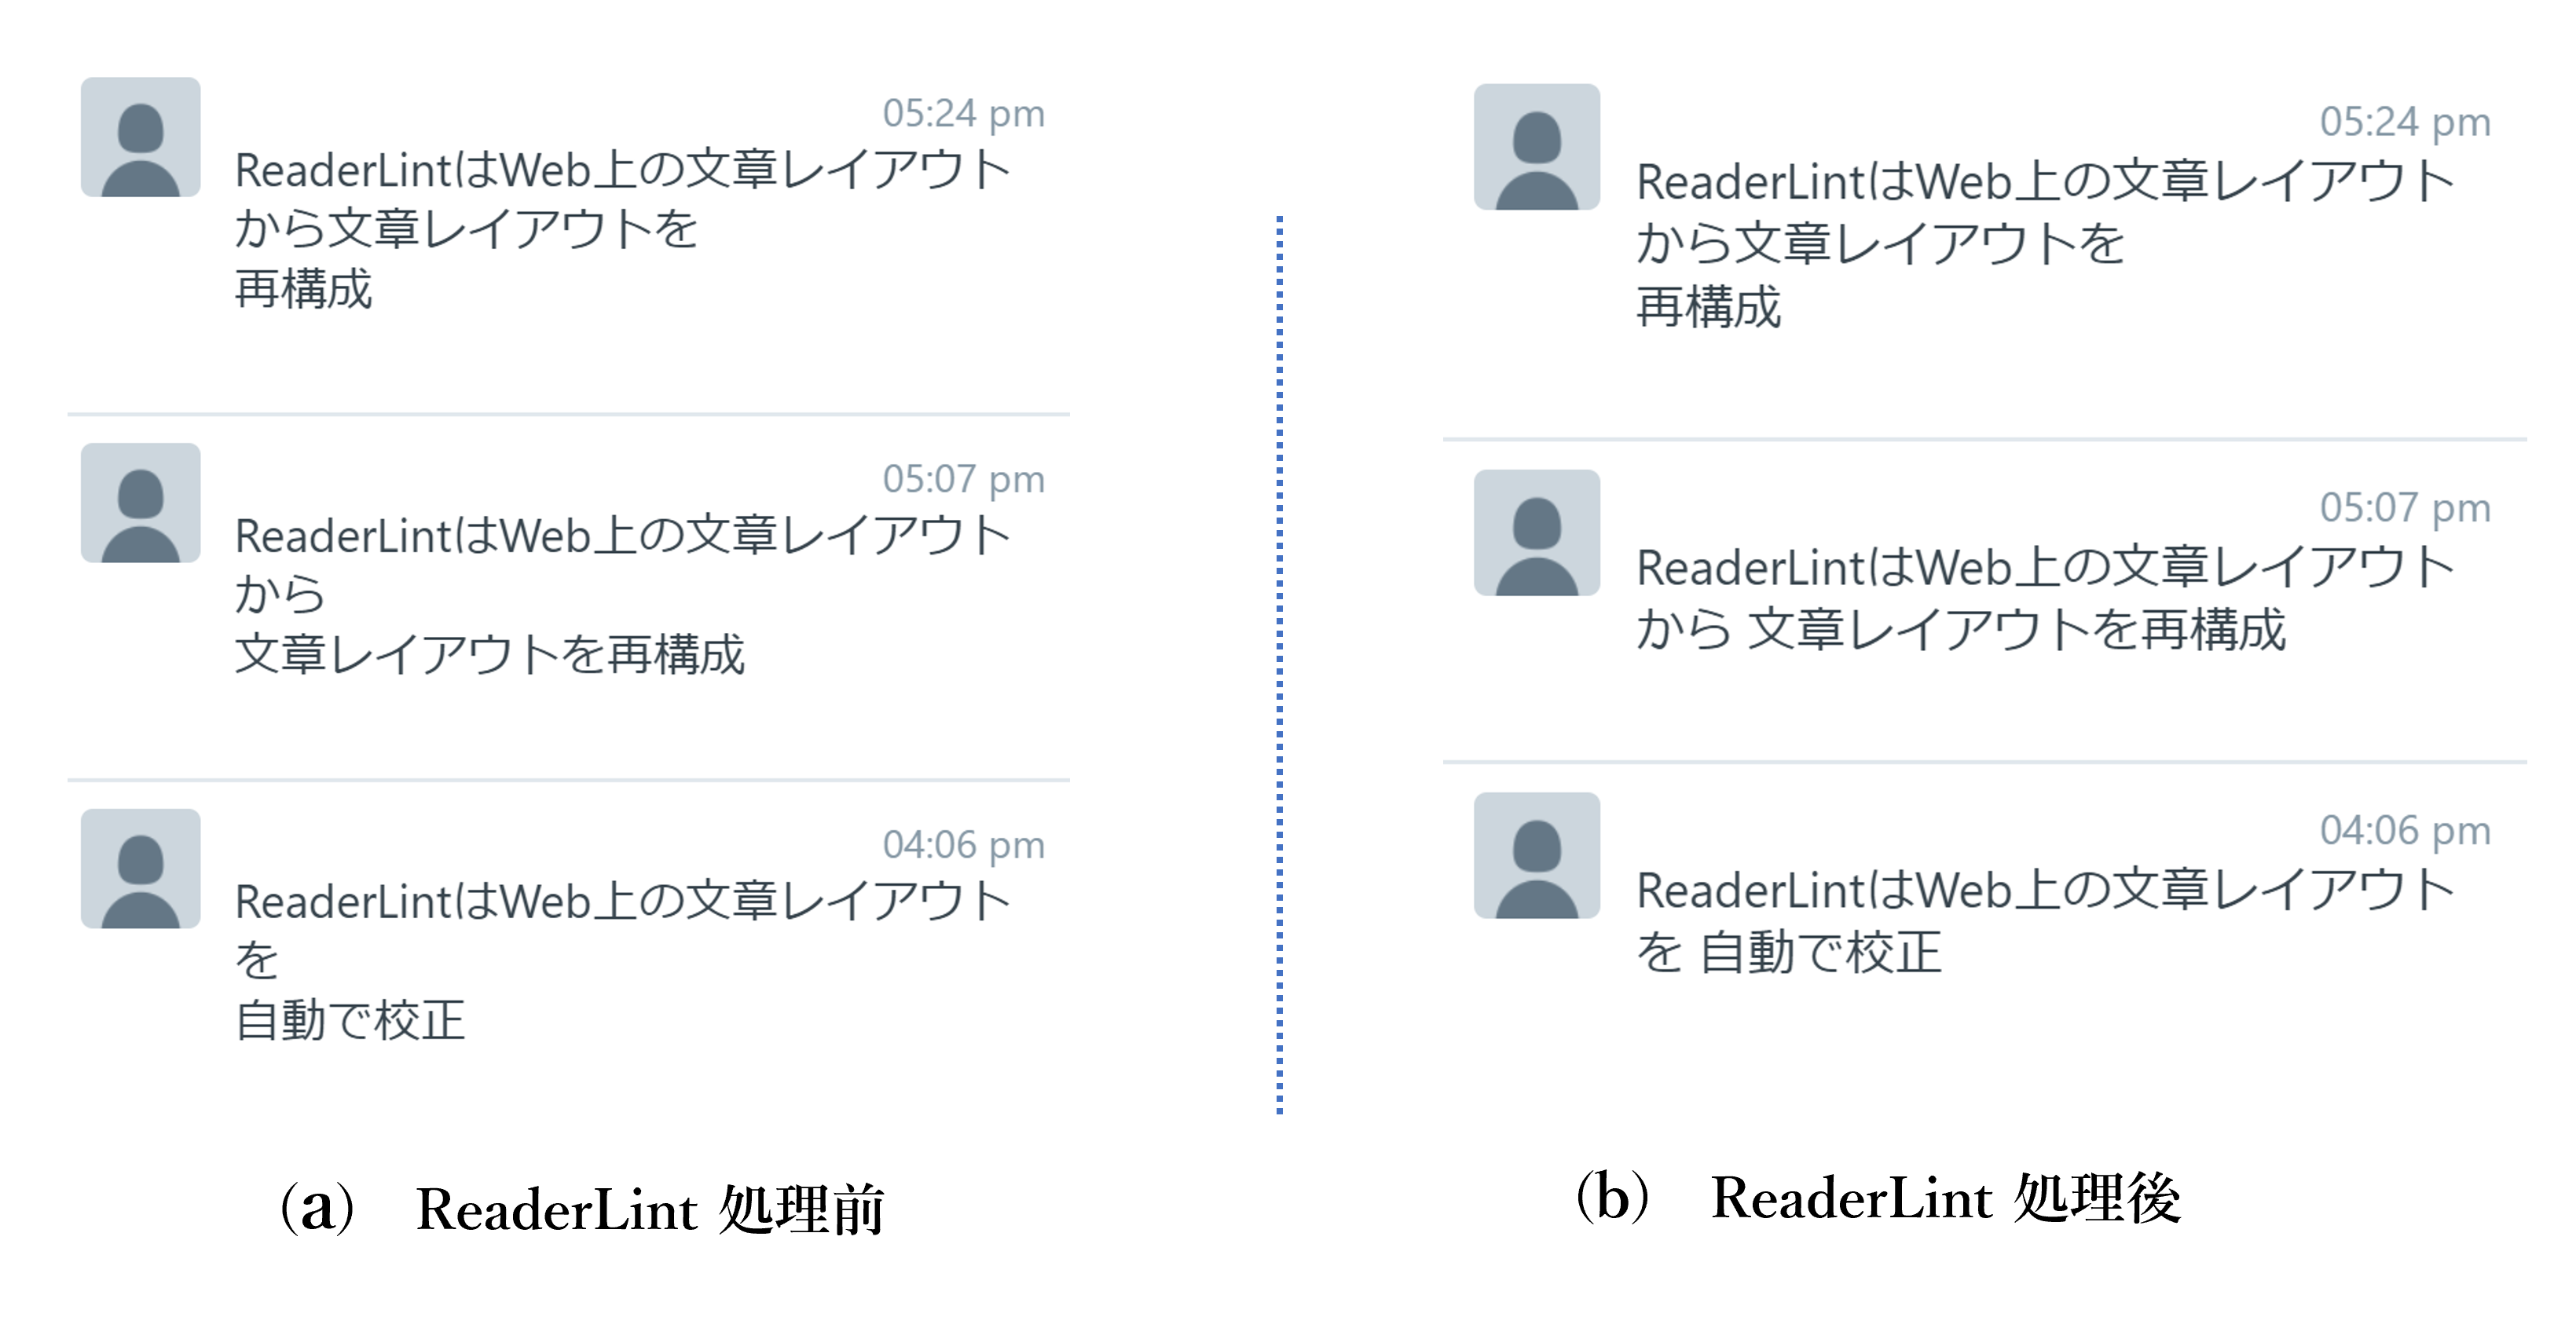
\includegraphics[width=0.7\columnwidth]{image/03/img10.png}
	\caption[字詰めを行なった図]{字詰めを行なった図}
\end{figure}

\subsection{ウィンドウサイズ変更による改行位置のズレの検出}
文節ごとの改行レイアウト処理を行なったあとDOMのサイズが変更した場合,
今回の実装形態の場合ではブラウザのウィンドウサイズが変更した際には文章の折返し箇所が変化するため,
文章レイアウトの崩れが発生する.

\begin{figure}[H]
    \centering
    \label{fig:resize}
    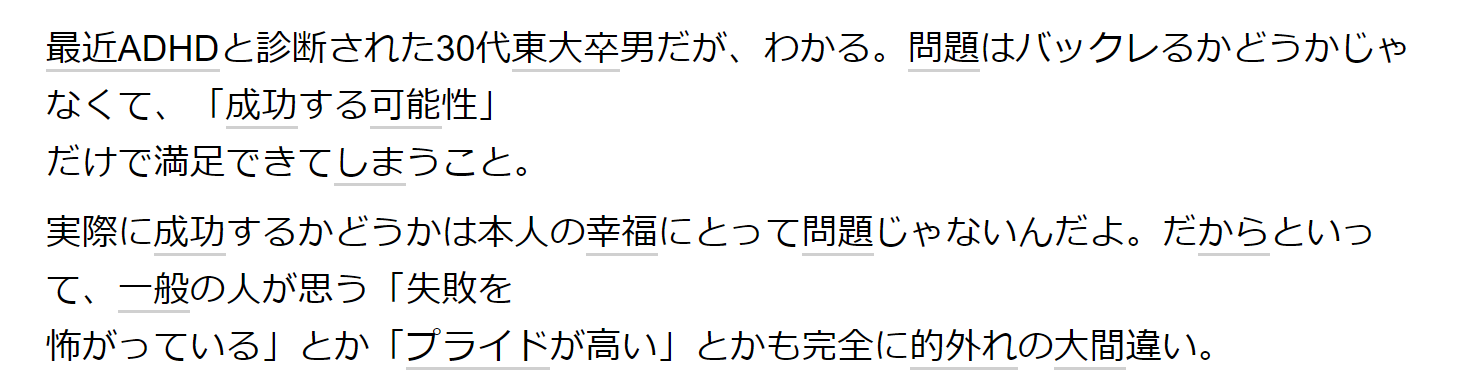
\includegraphics[width=0.7\columnwidth]{image/03/img9.png}
	\caption[ReaderLint後にウインドウサイズを変更した場合]{ReaderLint後にウインドウサイズを変更した場合}
\end{figure}

このようなケースへの対策のため.変更前に文章の文字列を新たに変更になったDOMの横幅をもとに改行レイアウト処理をかける必要がある.
今回はchrome localstorage内に,ReaderLintを実行したのタグデータ,クラス名,ReaderLintをかけた後の文字列をキー,
変化前の原文をvalueとしたJSONやDOMのクラス名,タグ等をJSON形式に格納した.これを用いてブラウザウインドウのサイズ変更を検知した際に
変更後のDOMのサイズから再び改行処理を加えることが可能となった.以下はデータ構造の本文該当箇所(innerHTMLの項目)を簡略化して表示したものである.
本来のデータはinnerHTMLの箇所には変更後の文章全文が追加されており,参照が可能となっている.

\newpage

\begin{lstlisting}
{
  "className": "js-tweet-text tweet-text with-linebreaks already",
  "tagName": "P",
  "url": "https://tweetdeck.twitter.com/",
  "innerHTML": {
    "吾輩は猫である。名前はまだ無い。\nどこで生れたかとんと見当がつかぬ...:"吾輩は猫である。名前はまだ無い。どこで生れたかとんと見当がつかぬ...
  }
}
\end{lstlisting}

\section{まとめ}
文章の視認性を上げるための要件定義を羅列し,その実装形態であるReaderLintと,その実装方法を述べた.
ブラウザ上に文章が生じされた後,対象となる文章をDOMとして指定し文章とそのDOMの設定を読み込む.文章の解析をASTとして行うことでブラウザ上に文字列して表示される要素と直接は描画されないHTML要素を分け,
TinySegmenterによって分かち書きされた文節ごとに描画幅を計測した行頭から幅を加算していき,総和がDOMの幅を超過すると予想された文節箇所の前に改行を追加する処理を入れることで文節間改行レイアウトを実装した.
